\chapter{Resultados}
\label{cap:resultados}
En este capítulo se presentan los resultados obtenidos tras la ejecución del plan de pruebas propuesto en el capítulo anterior.

\section{Evalución algorítmica}

\subsection{Convergencia}
El algoritmo memético hace uso de un control de reinicio que se adapta según el tiempo que le toma en cada convergencia. Tras converger, guarda la cantidad de generaciones \textit{G} que le tomó estancarse y se reinicia la población según el algoritmo \ref{alg:memetico-restart}, luego el MA tiene G generaciones para poder encontrar una mejor solución antes de volver a reiniciar la población. A continuación, se exponen los gráficos de convergencia del algoritmo para cada una de las 6 proteínas probadas en este trabajo. Se puede apreciar la contribución de los reinicios de la población al resultado final que entrega el MA. Los gráficos expuestos corresponden a las ejecuciones que entregaron las energías más bajas para cada proteína.

\begin{figure}
\centering
\begin{tabular}{c c}
\\
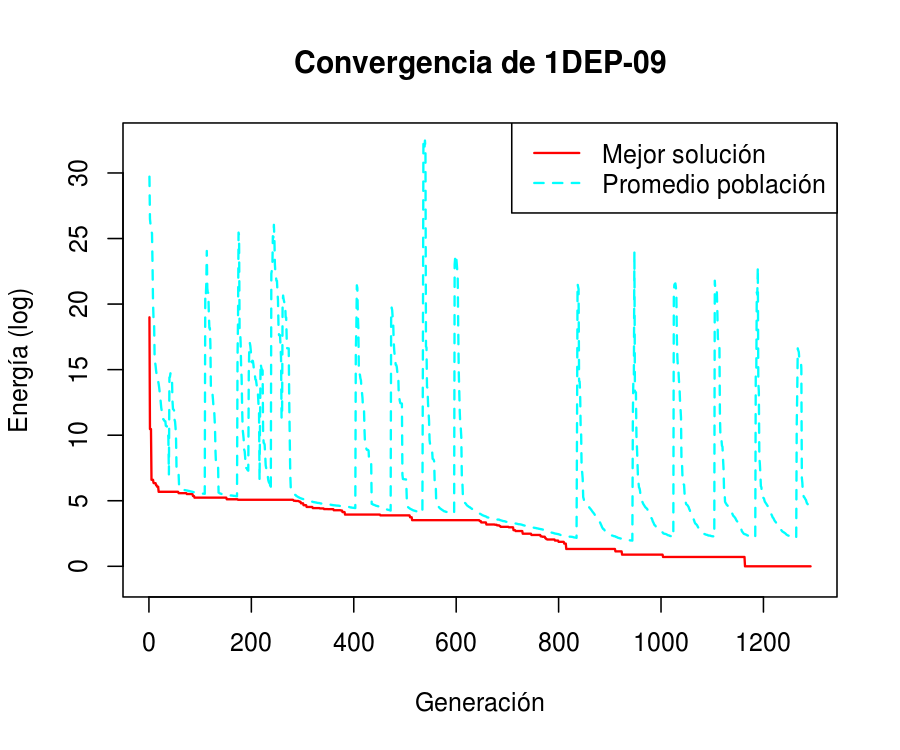
\includegraphics[height=6cm]{images/convergencia-1DEP-09.png} & 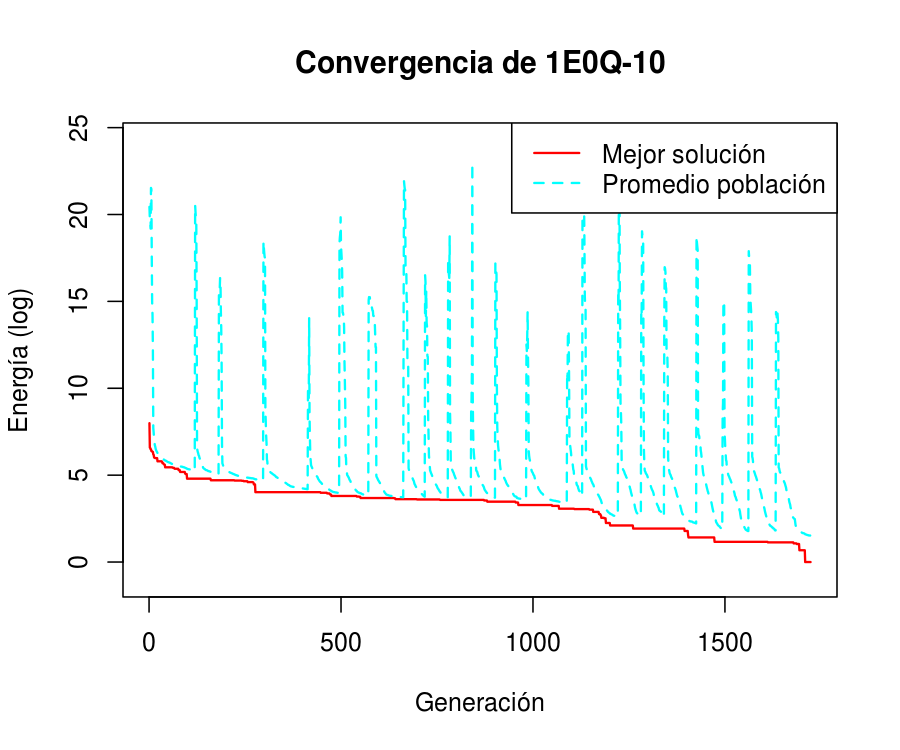
\includegraphics[height=6cm]{images/convergencia-1E0Q-10.png} \\
(a) & (b) \\
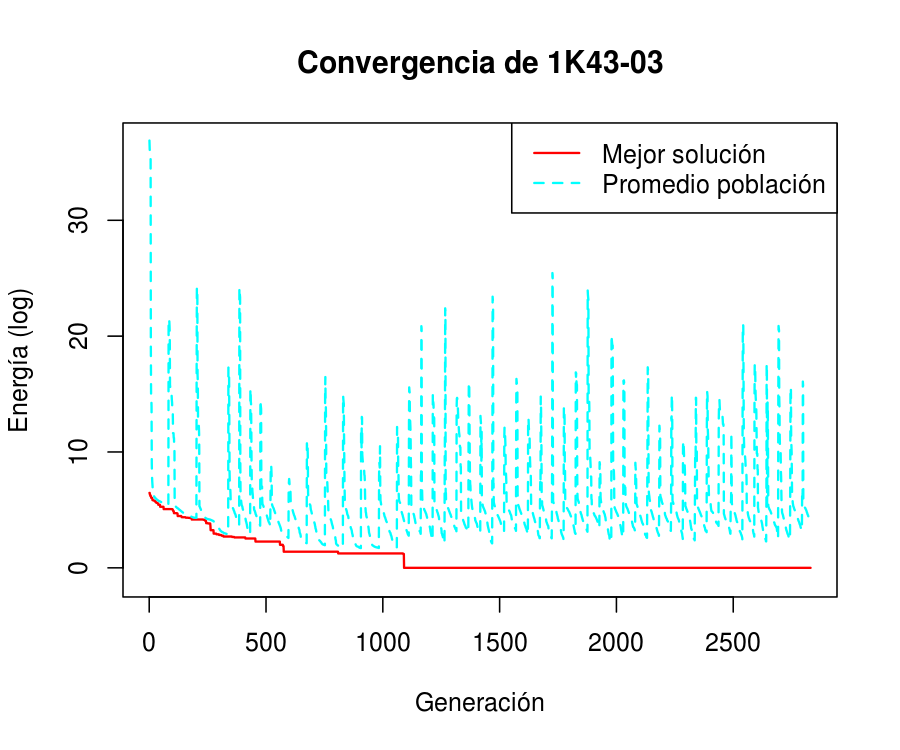
\includegraphics[height=6cm]{images/convergencia-1K43-03.png} & 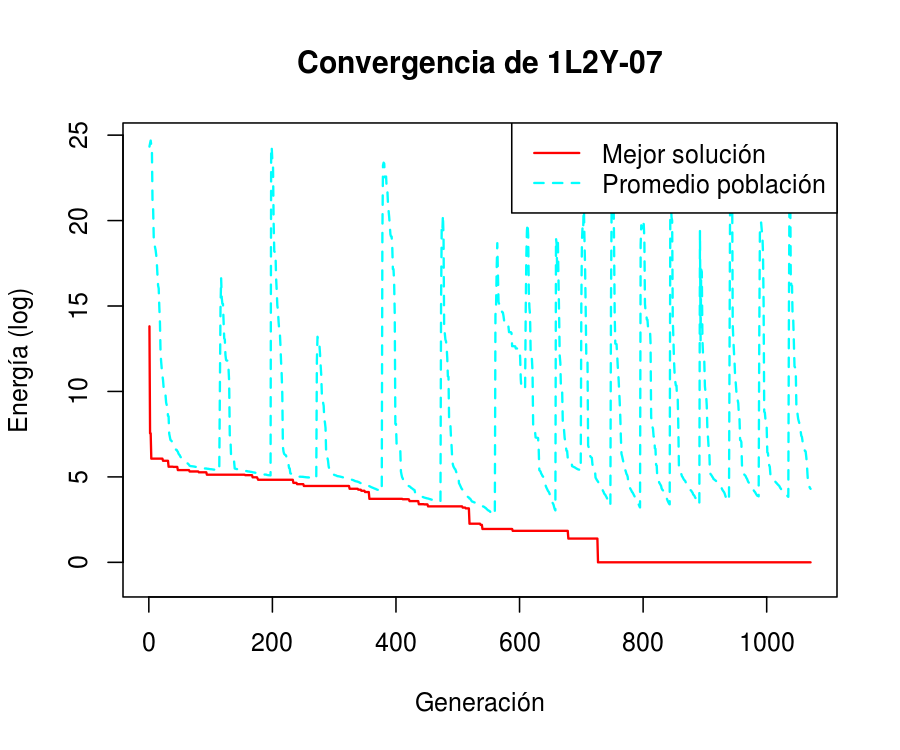
\includegraphics[height=6cm]{images/convergencia-1L2Y-07.png} \\
(c) & (d) \\
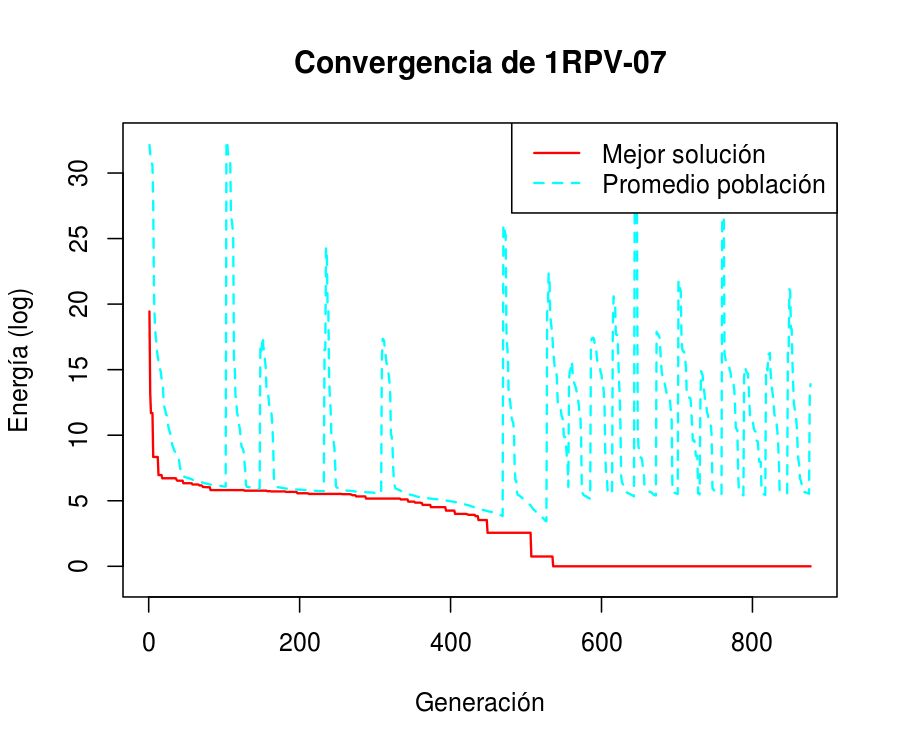
\includegraphics[height=6cm]{images/convergencia-1RPV-07.png} & 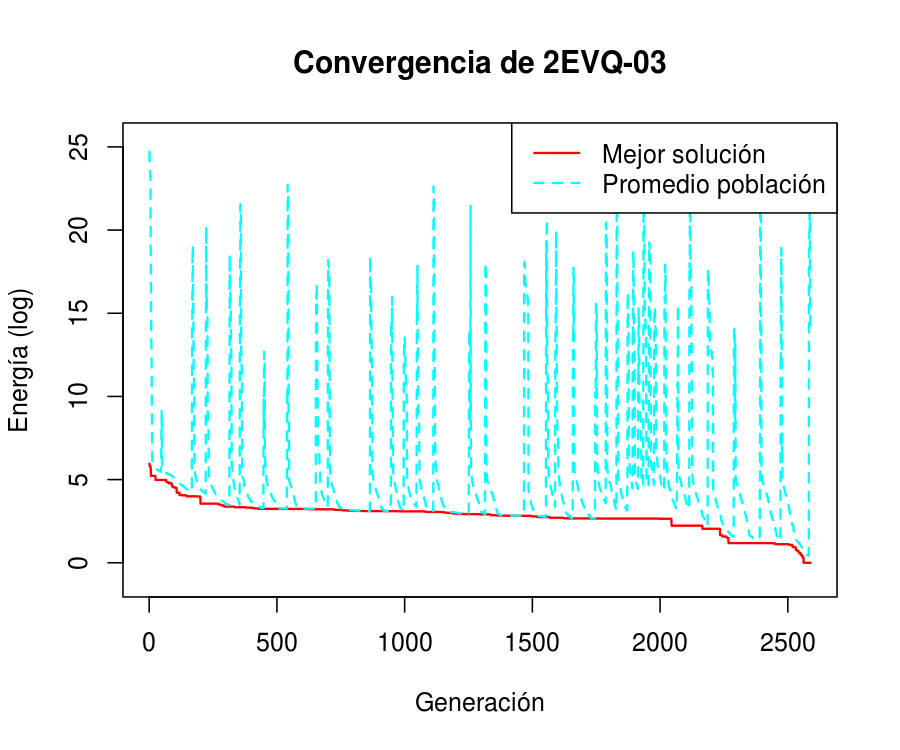
\includegraphics[height=6cm]{images/convergencia-2EVQ-03.png} \\
(e) & (f) \\

\end{tabular}
\caption[Curvas de convergencia]{Ejemplos de curvas de convergencia del algoritmo mem\'etico para las proteinas (a) 1DEP, (b) 1E0Q, (c) 1K43, (d) 1L2Y, (e) 1RPV y (f) 2EVQ}
\label{fig:convergencia}
\end{figure}

En la figura \ref{fig:convergencia} se puede observar la contribución del control de reinicio a la mejor solución al enfrentarse con la convergencia de la población de agentes. Por otra parte, existen casos con problemas de convergencia en sus últimas generaciones (gráfico (c) figura \ref{fig:convergencia}  de la generación 1000 en adelante), una forma de solucionar este problema podría ser mediante la implementación de un control de reinicio completo de la población (sin preservación de soluciones).


\subsection{Parámetros}
Los parámetros usados para la experimentación fueron establecidos tras pruebas de corta duración (1 a 3 horas) a medida que se realizaba la implementación del MA, haciendo uso delas proteínas 1K43 y 1L2Y, ya que estas presentas zonas de díficil predicción (hojas-$\beta$ y vueltas). No fue posible realizar una parametrización más rigurosa debido al tiempo del que se disponía para la construcción y implementación del MA. Los parámetros usados en las pruebas están presentes en la tabla \ref{table:lista-valores-parametros}.

\begin{table}[h]
	\centering
	\caption{Parámetros usados en las pruebas}
	\begin{tabular}{|l|r|}
		\hline
		Parámetro & Valor \\ \hline
		MAX\_SECS 	& 86400		\\		
		MAX\_GENS\_NOIMPROVE 	& 20		\\ 		
		LS\_PROB 	& 0.9		\\  	
		DIVERSITY 	& 10.0		\\ 		
		CROSSOVER 	& 0.4		\\ 		
		MUT\_ADJUSTMENT 	& 0.05		\\ 		
		MUT\_PROB 	& 0.5		\\		
		JUMP\_PROB 	& 0.3		\\		
		JUMP\_RADIUS 	& 90		\\		
		JUMP\_FACTOR 	& 0.85		\\	\hline	
	\end{tabular}
	\label{table:lista-valores-parametros}
\end{table}

\section{Calidad biológica de las soluciones}

\subsection{Contribución APL}

La tabla \ref{table:results-apl-noapl} muestra el resumen de los resultados generados por el Algoritmo Memético que hace uso de la APL en contraste cuando obtiene valores aleatorios para los ángulos de torsión.

\begin{table}[h]
	\centering
	\caption[Análisis comparativo de resultados de APL y Sin APL]{Análisis comparativo de resultados obtenidos de MA con APL y sin APL. Energía medida en $Kcal/mol$ y RMSD medido en $\AA$}
\begin{tabularx}{\textwidth}{|l|r|r|r|r|r|r|} \hline
{PDB} & \multicolumn{2}{c|}{APL} & \multicolumn{2}{c|}{Sin APL} & \multicolumn{2}{c|}{\textit{p-value}}\\ \cline{2-7}
 {ID} & \multicolumn{1}{c|}{Energía} & \multicolumn{1}{c|}{RMSD} & \multicolumn{1}{c|}{Energía} & \multicolumn{1}{c|}{RMSD} & \multicolumn{1}{c|}{Energía} & \multicolumn{1}{c|}{RMSD} \\ \hline
 {2EVQ} & -94.2 (-70.2) & 3.58 (2.87) & -92.6 (-40.8) & 3.76 (2.76) & $8.398^{-2}$ & $4.922^{-1}$   \\
 {1K43} & -558.6 (-515.2) & 2.50 (2.71) & -447.8 (-405.0) & 5.05 (4.77 ) & $\mathbf{1.953^{-3}}$ & $\mathbf{1.953^{-3}}$\\
 {1DEP} & -304.2 (-272.7) & 1.43 (1.03) & -377.3 (-239.2)  & 4.12 (4.28) & $3.750^{-1}$ & $\mathbf{5.889^{-3}}$\\
 {1E0Q} & -280.9 (-236.7) & 7.08 (4.77) & -141.2 (-49.4) & 5.04 (5.41 ) & $\mathbf{1.953^{-3}}$ & $4.922^{-1}$  \\
 {1RPV} & -1027.9 (-937.3) & 2.15 (1.88) & -1075.1 (-947.3) & 5.66 (5.66 ) & $5.566^{-1}$ & $\mathbf{1.953^{-3}}$  \\
 {1L2Y} & -261.9 (-225.7) & 5.43 (4.04) & -187.4 (-23.8) & 5.01 (5.39 ) & $\mathbf{1.953^{-3}}$ & $\mathbf{9.766^{-3}}$ \\ \hline
\end{tabularx}
\label{table:results-apl-noapl}
\end{table}

Para validar estadísticamente estos resultados, la columna \textit{p-value} de la tabla \ref{table:results-apl-noapl} muestra los valores arrojados por el test de Wilcoxon que se utiliza para comparar dos mediciones de rangos y determinar que la diferencia no se deba al azar. Dado dichos resultados, se comprueba estadísticamente que la contribución de la APL es estadísticamente significativa.


\subsection{Análisis RMSD}

La tabla \ref{table:results-summary} muestra el resumen de las 10 ejecuciones del MA sobre cada secuencia. El MA es capaz de alcanzar bajos valores de energía mientras a la vez alcanza buenas soluciones en términos de RMSD. Las imágenes de la figura \ref{fig:rmsd-proteinas} muestran las comparaciones realizadas mediante la alineación espacial de las soluciones con mejor RMSD, mejor energía y la estructura experimental correspondiente.

\begin{table}[h]
\small
\centering
\caption[Resumen de resultados]{Resumen de resultados usando APL, tomando las mejores soluciones obtenidas por el MA desde el punto de vista RMSD y energía.}
\scalebox{1}{
\begin{tabular}{|c|r|r|c|c|r|r|} \hline
\multirow{2}{*}{PDB} & \multicolumn{1}{c|}{Menor} & \multicolumn{1}{c|}{Promedio} & \multicolumn{1}{c|}{RMSD (\AA)} & \multirow{1}{*}{Menor}& \multirow{1}{*}{Promedio} & \multicolumn{1}{c|}{Promedio}\\

\multirow{2}{*}{ID} & \multicolumn{1}{c|}{Energía} & \multicolumn{1}{c|}{Energía} & \multicolumn{1}{|c|}{Menor} & \multirow{1}{*}{RMSD (\AA)}& \multirow{1}{*}{RMSD (\AA)} & \multicolumn{1}{c|}{Número de}\\

 & \multicolumn{1}{c|}{($\text{Kcal}/\text{mol}^{-1}$)} & \multicolumn{1}{c|}{($\text{Kcal}/\text{mol}^{-1}$)} & \multicolumn{1}{c}{Energía} & \multicolumn{1}{|c|}{} & \multicolumn{1}{|c|}{} & \multicolumn{1}{c|}{Generaciones}\\
\hline
{2EVQ} & -94.21  & -70.24 ($\pm$14.69)   & 3.58   & 1.35  & 2.87 ($\pm$0.84)  & 3760.3\\\hline
{1K43} & -558.56  & -515.16 ($\pm$36.40)   & 2.50   & 1.27  & 2.71 ($\pm$0.83)  & 2536.8\\\hline
{1DEP} & -304.16  & -272.69 ($\pm$24.42)   & 1.43   & 0.39  & 1.03 ($\pm$0.44)  & 1414.3\\\hline
{1E0Q} & -280.86  & -236.72 ($\pm$32.21)   & 7.08   & 2.21  & 4.77 ($\pm$2.1)  &  1389.8\\\hline
{1RPV} & -1027.95  & -937.26 ($\pm$76.88)   & 2.15   & 0.97  & 1.88 ($\pm$0.46)  & 834.5\\\hline
{1L2Y} & -261.90  & -225.65 ($\pm$32.36)   & 5.43   & 2.26  & 4.04 ($\pm$1.10)  & 1027.1\\\hline
\end{tabular}}\label{table:results-summary}
\end{table}



\begin{figure}
\centering
\begin{tabular}{c c}
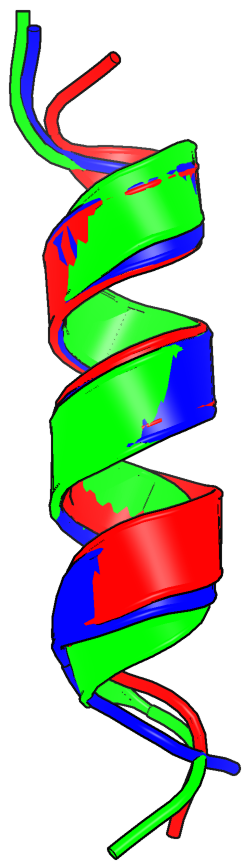
\includegraphics[height=5.2cm]{images/rmsd-1DEP.png} & 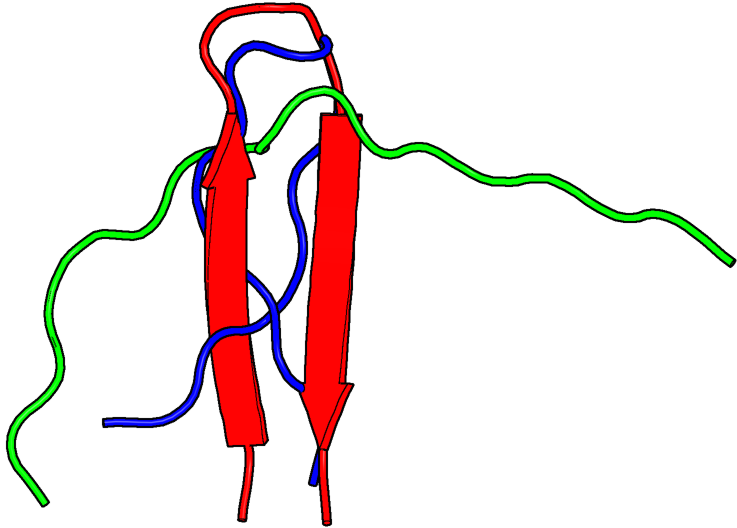
\includegraphics[height=5.2cm]{images/rmsd-1E0Q.png} \\
(a) & (b) \\ \\
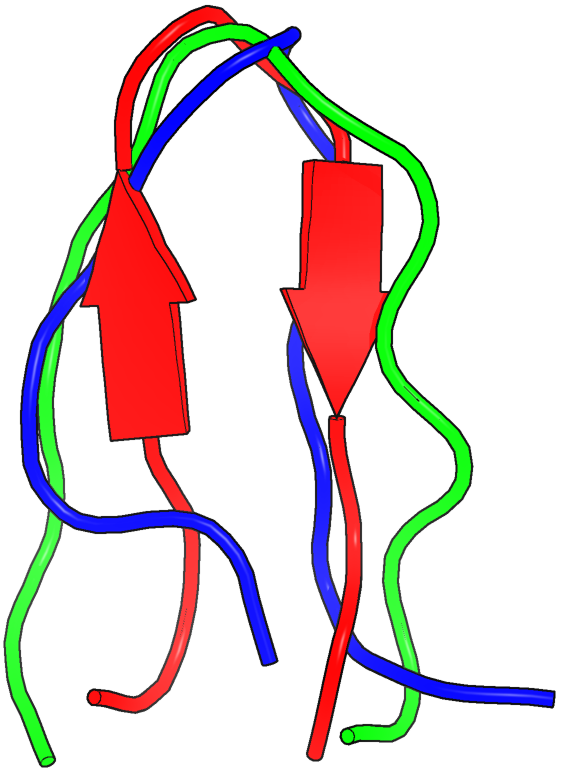
\includegraphics[height=5.2cm]{images/rmsd-1K43.png} & 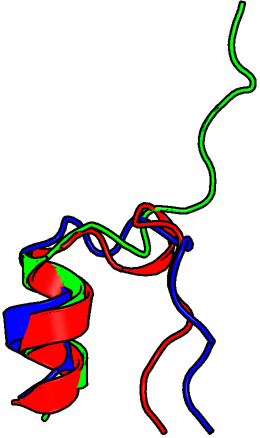
\includegraphics[height=5.2cm]{images/rmsd-1L2Y.png} \\
(c) & (d) \\ \\
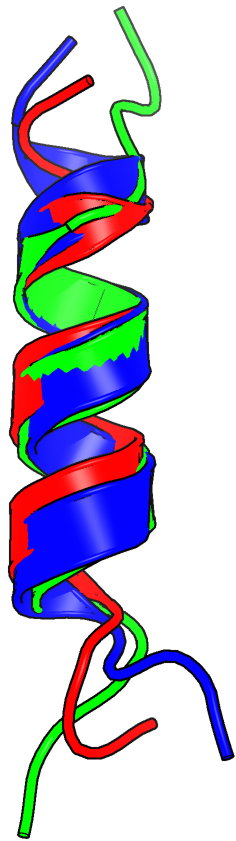
\includegraphics[height=5.2cm]{images/rmsd-1RPV.png} & 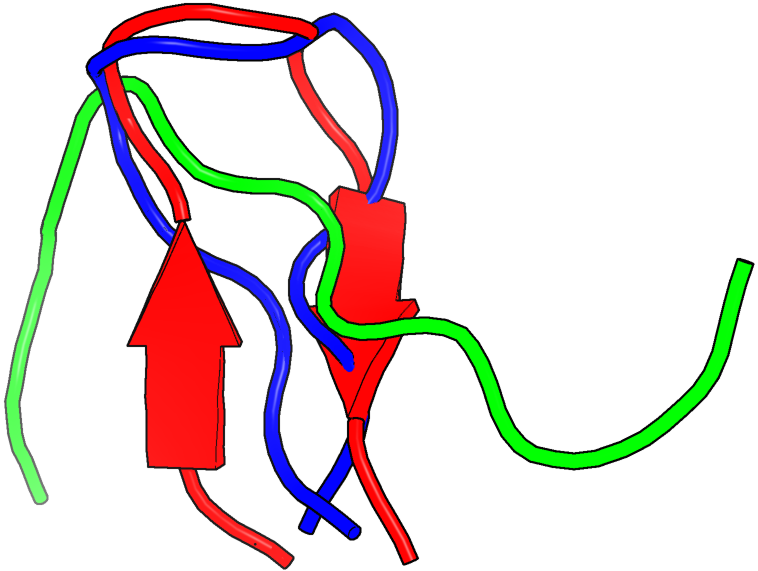
\includegraphics[height=5.2cm]{images/rmsd-2EVQ.png} \\
(e) & (f) \\

\end{tabular}
\caption[Alineación espacial de estructuras]{Resultados de alineación espacial para las proteínas (a) 1DEP, (b) 1E0Q, (c) 1K43, (d) 1L2Y, (e) 1RPV y (f) 2EVQ. Solución con mejor energía en color verde, mejor RMSD en azul y estrcutura experimental en rojo. Las estructuras fueron alineadas a partir de la superposición de sus $C_{\alpha}$ utilizando PyMol.}
\label{fig:rmsd-proteinas}
\end{figure}


Es importante recordar que el usar la energía como función de minimización \textbf{no garantiza que la mejor solución en términos de energía tendrá el mejor RMSD} cuando se compare con la proteína experimental. En la tabla \ref{table:results-summary} la mejor solución en términos de RMSD no corresponde a la solución que obtiene la energía más baja.

\subsection{Análisis de estructura secundaria}

La tabla \ref{table:stridess} compara las estructuras secundarias de las soluciones obtenidas por el algoritmo contra las proteínas experimentales. 

\begin{table}[H]
\centering
\caption[Resultados PROMOTIF]{Resultados de PROMOTIF para las estructuras experimentales (E) y soluciones con menor energía (P).}

\begin{tabular}{|l|r|r|r|r|}\hline
{PDB ID} & \% hojas-$\beta$ & \% hélices-$\alpha$ & \% hélices-$3^{10}$ & \% Otras\\\hline

2EVQ-E & 50 & 0 & 0 & 50\\
2EVQ-P & 0 & 0 & 0 & 100\\\hline

1K43-E & 43  & 0 & 0 & 57\\
1K43-P & 0 & 0 & 0 & 100\\\hline

1DEP-E & 0 & 80 & 0 & 20\\
1DEP-P & 0 & 54 & 13 & 33\\\hline

1E0Q-E & 71 & 0 & 0 & 29\\
1E0Q-P & 0 & 0 & 0 & 100\\\hline

1RPV-E & 0 & 65 & 0 & 35\\
1RPV-P & 0 & 59 & 0 & 41\\\hline

1L2Y-E & 0 & 35 & 20 & 45\\
1L2Y-P & 0 & 40 & 0 & 60\\\hline
\end{tabular}
\label{table:stridess}
\end{table}

Este análisis revela que la topología de las soluciones predichas y las experimentales son comparables a las estructuras experimentales. En general, el MA propuesto tiene problemas en la predicción de hojas-$\beta$ y áreas de curvatura (se puede apreciar en la tabla \ref{table:stridess} en las proteínas 2EVQ, 1k43 y 1E0Q), no así con la predicción de hélices (ver proteínas 1RPV, 1DEP y 1L2Y).  

\subsection{Análisis Estereoquímico}

La tabla \ref{table:procheck} resume numéricamente los valores del gráfico de Ramachandran para las proteínas experimentales y estructuras predichas.

\begin{table*}[!htb]
\centering
\caption{Valores de los gráficos de Ramachadran para las estructuras experimentales(E) y predichas(P) usando PROCHEK.}
\scalebox{1}{
\begin{tabular}{|l|r|r|r|r|r|} \hline
\multirow{2}{*}{PDB ID}   &   \multirow{2}{*}{Most  Favorable}     & \multirow{2}{*}{Most Allowed}    & \multirow{2}{*}{Generously Allowed} &  \multirow{2}{*}{Disallowed} & \multicolumn{1}{l|}{N. amino}\\
   &      &      &  &   & \multicolumn{1}{c|}{acid Res.}\\\hline
2EVQ-E  & 7~(87.5\%)   & 1~(12.5\%) & 0~(0.0\%) & 0~(0.0\%) & 8\\
2EVQ-P  & 7~(87.5\%)  & 1~(12.5\%)  & 0~(0.0\%) & 0~(0.0\%) & 8\\\hline
1K43-E  & 6~(66.7\%)   & 3~(33.3\%) & 0~(0.0\%) & 0~(0.0\%) & 9\\
1K43-P  & 8~(88.9\%)  & 1~(11.1\%)  & 0~(0.0\%) & 0~(0.0\%) & 9\\\hline
1DEP-E  & 11~(91.7\%)   & 1~(8.3\%) & 0~(0.0\%) & 0~(0.0\%) & 12\\
1DEP-P  & 11~(91.7\%)  & 0~(0.0\%)  & 1~(8.3\%) & 0~(0.0\%) & 12\\\hline
1E0Q-E  & 14~(100.0\%)   & 0~(0.0\%) & 0~(0.0\%) & 0~(0.0\%) & 14\\
1E0Q-P  & 13~(92.9\%)  & 1~(7.1\%)  & 0~(0.0\%) & 0~(0.0\%) & 14\\\hline
1RPV-E  & 13~(86.7\%)   & 2~(13.3\%) & 0~(0.0\%) & 0~(0.0\%) & 15\\
1RPV-P  & 14~(93.3\%)  & 1~(6.7\%)  & 0~(0.0\%) & 0~(0.0\%) & 15\\\hline
1L2Y-E  & 10~(90.9\%)   & 1~(9.1\%) & 0~(0.0\%) & 0~(0.0\%) & 11\\
1L2Y-P  & 11~(100.0\%)  & 0~(0.0\%)  & 0~(0.0\%) & 0~(0.0\%) & 11\\\hline
\end{tabular}}\label{table:procheck}
\end{table*}

Se observa que en todas las estructuras predichas, los residuos de aminoácidos están localizados en las regiones más favorables del mapa. La configuración esteroquímica de la molécula de una proteína está determinada por la relación de los átomos en el espacio tridimensional, las soluciones predichas tienen cerca del $90\%$ de sus residuos en las regiones más favorables lo que significa que tienen alta calidad estereoquímica. Cuando se compara los resultados obtenidos por el método propuesto con los datos experimentales, se observa que estas estructuras son comparables en terminos de calidad estereoquímica.

\section{Comportamiento con proteínas extensas}

La tabla \ref{tab:prot-ext-summary} muestra los mejores resultados paralas 9 proteínas predichas en terminos de RMSD y energía. Dichos resultados se pueden visualizar en las figuras \ref{fig:prot-ext-1} y \ref{fig:prot-ext-2}.

\begin{table}[H]
\centering
\caption[Resumen de resultados para proteínas extensas]{Resumen de resultados usando APL, tomando las mejores soluciones obtenidas por el MA desde el punto de vista RMSD y energía para las 9 proteínas propuestas.}
\begin{tabularx}{\textwidth}{|X|r|r|r|r|r|}
\hline
 \multirow{2}{*}{PDB ID} & \multicolumn{2}{c|}{Mejor Energía} & \multicolumn{2}{c|}{Mejor RMSD} & \multirow{2}{*}{Generaciones} \\ \cline{2-5}
 & Energía & RMSD & Energía & RMSD & \\ \hline
 
 2F4K & -696.124 & 6.879 & -667.282 & 6.85 & 630\\
 2JUC & 554.577 & 16.872 & 1.254.361 & 14.959 & 150\\
 2MR9 & -862.438 & 13.849 & -820.141 & 13.777 & 390\\
 2P5K & 426.634 & 25.818 & 921.558 & 10.877 & 137\\
 2P81 & -1.158.266 & 11.592 & -981.857 & 10.011 & 291\\
 3P7K & -800.774 & 1.786 & -648.753 & 1.439 & 296\\
 3V1A & -707.860 & 4.355 & -705.510 & 3.788 & 258\\
 2MQ8 & 104350.553 & 31.537 & 1.361.364.901 & 21.416 & 36\\
 2MW1 & 5817.577 & 21.911 & 17.602.208 & 20.565 & 42\\
 
\hline 
\end{tabularx}
\label{tab:prot-ext-summary}
\end{table}



\begin{figure}
\centering
\begin{tabular}{c c}
\\
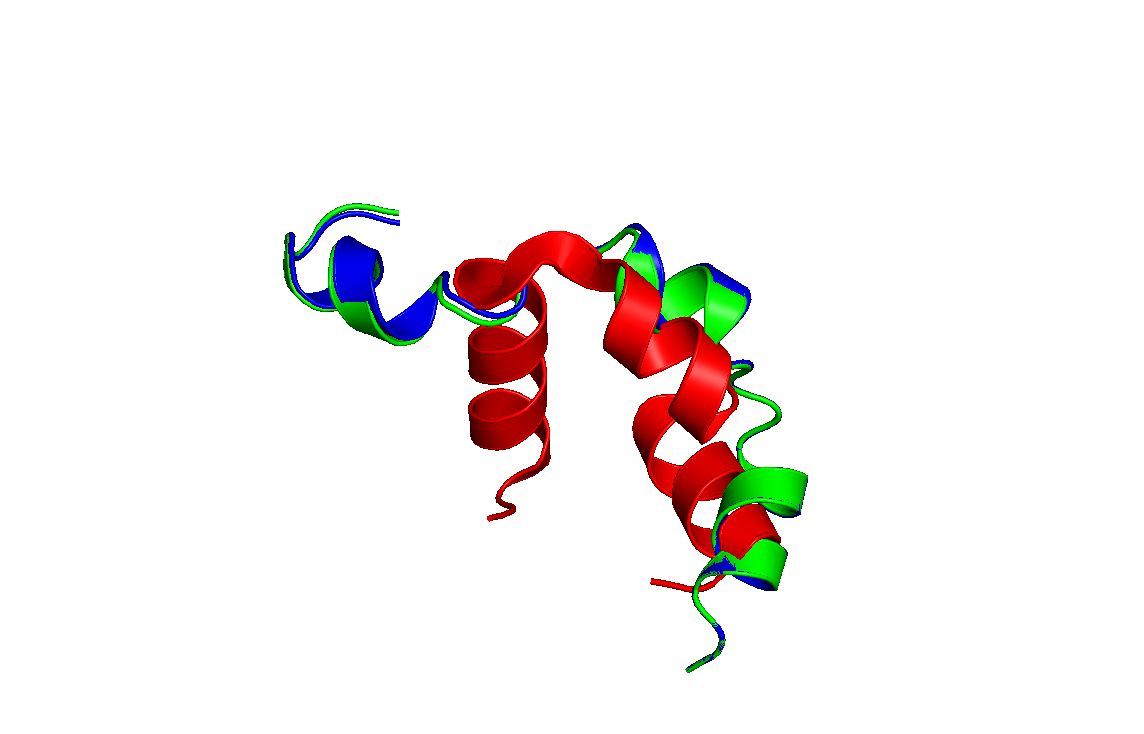
\includegraphics[width=8.5cm]{images/2F4K.png} & 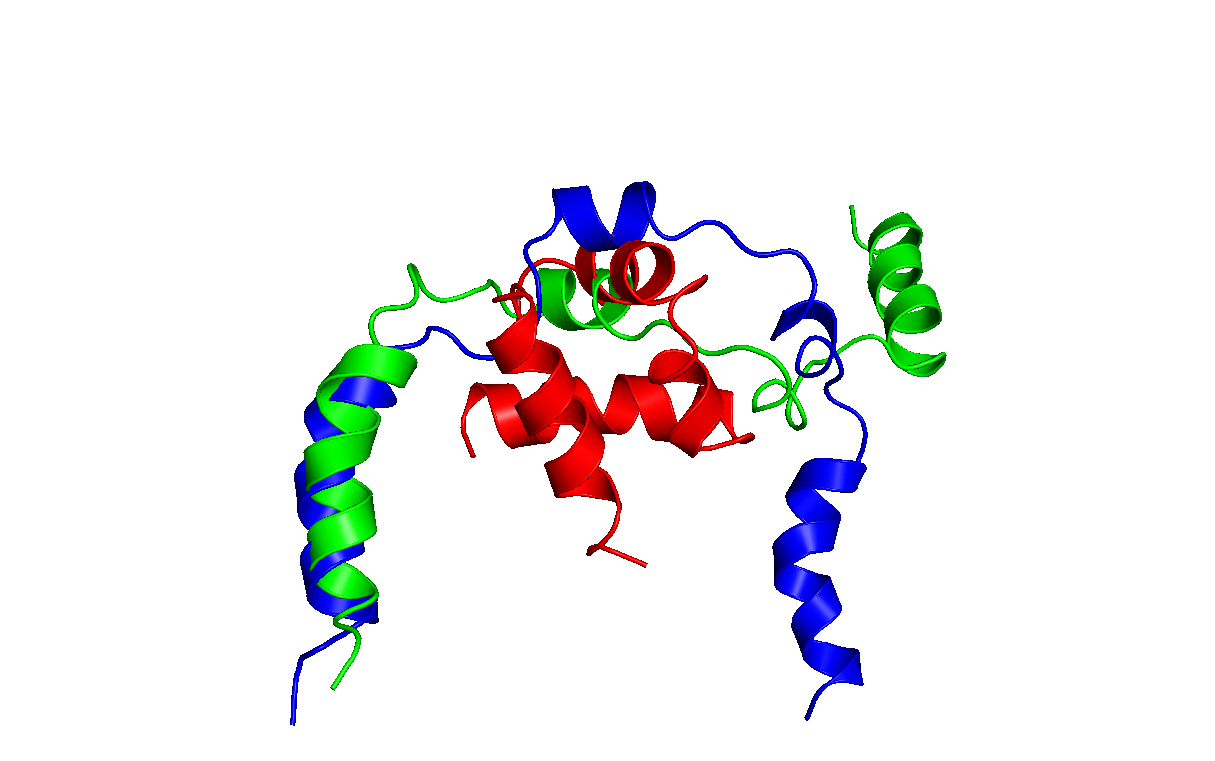
\includegraphics[width=8.5cm]{images/2JUC.png} \\
(a) & (b)\\
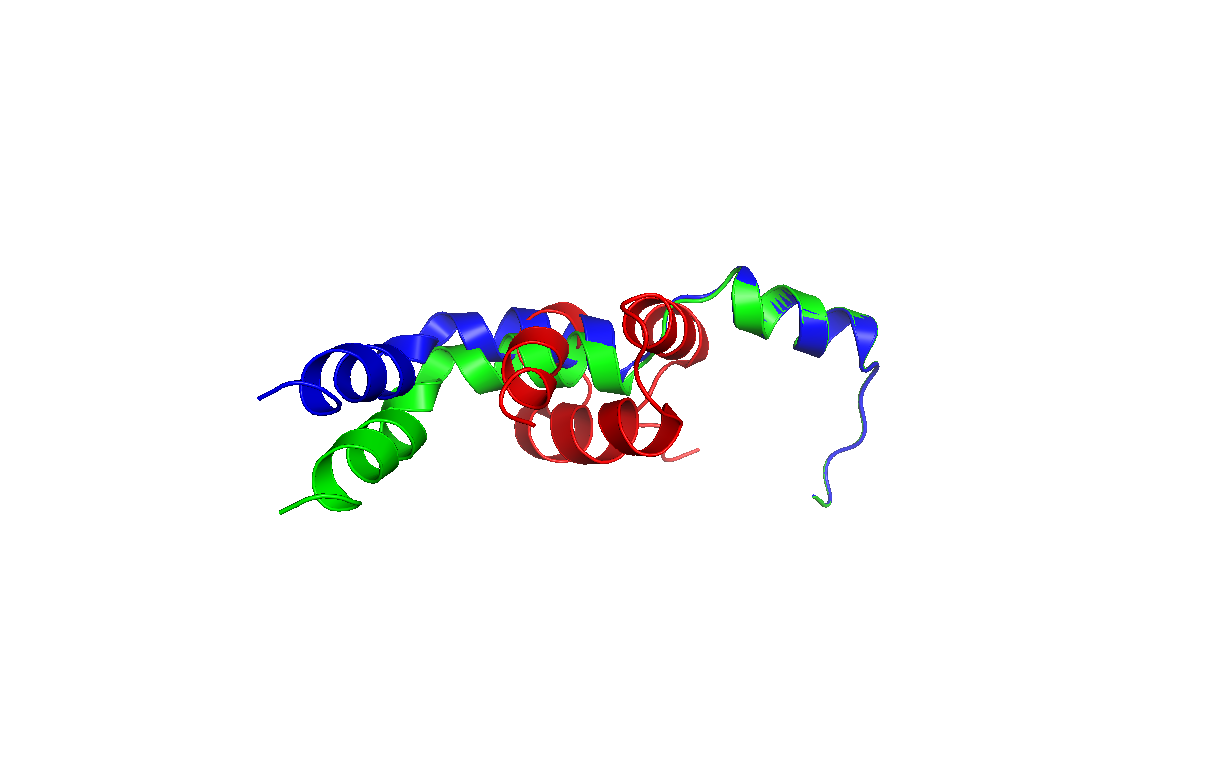
\includegraphics[width=8.5cm]{images/2MR9.png} & 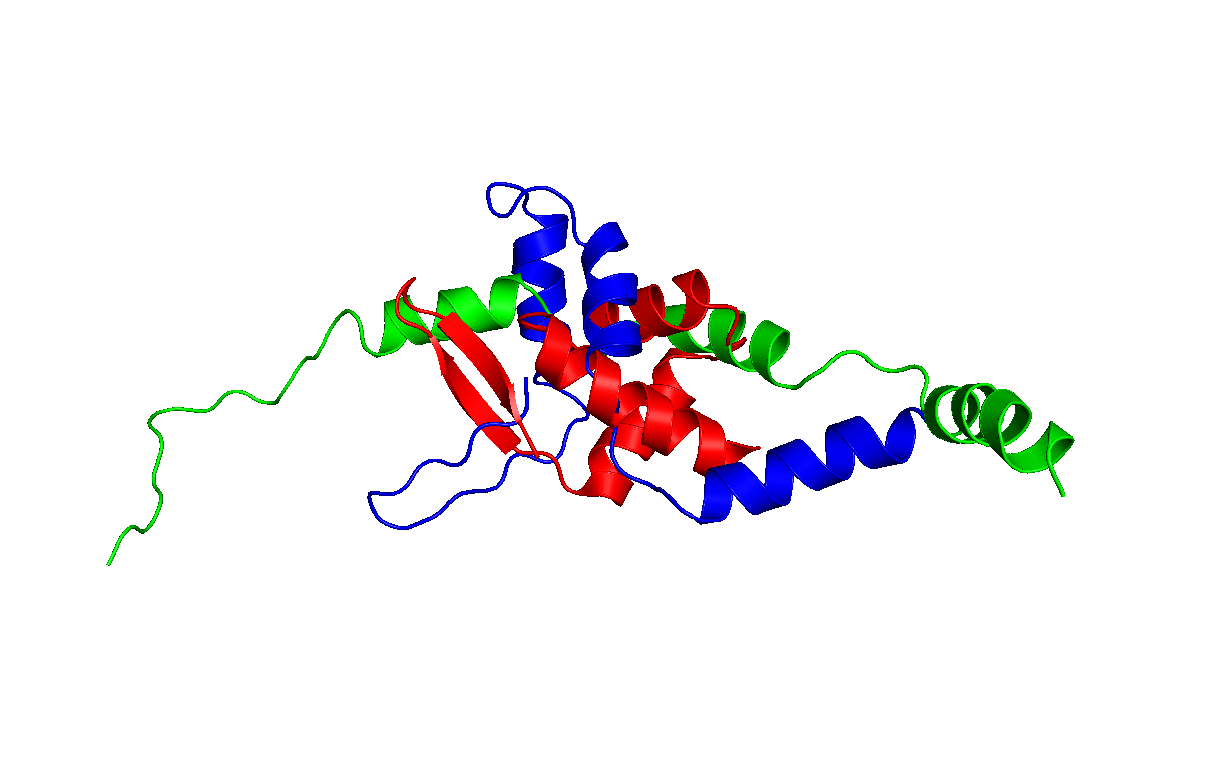
\includegraphics[width=8.5cm]{images/2P5K.png} \\
(c) & (d)\\
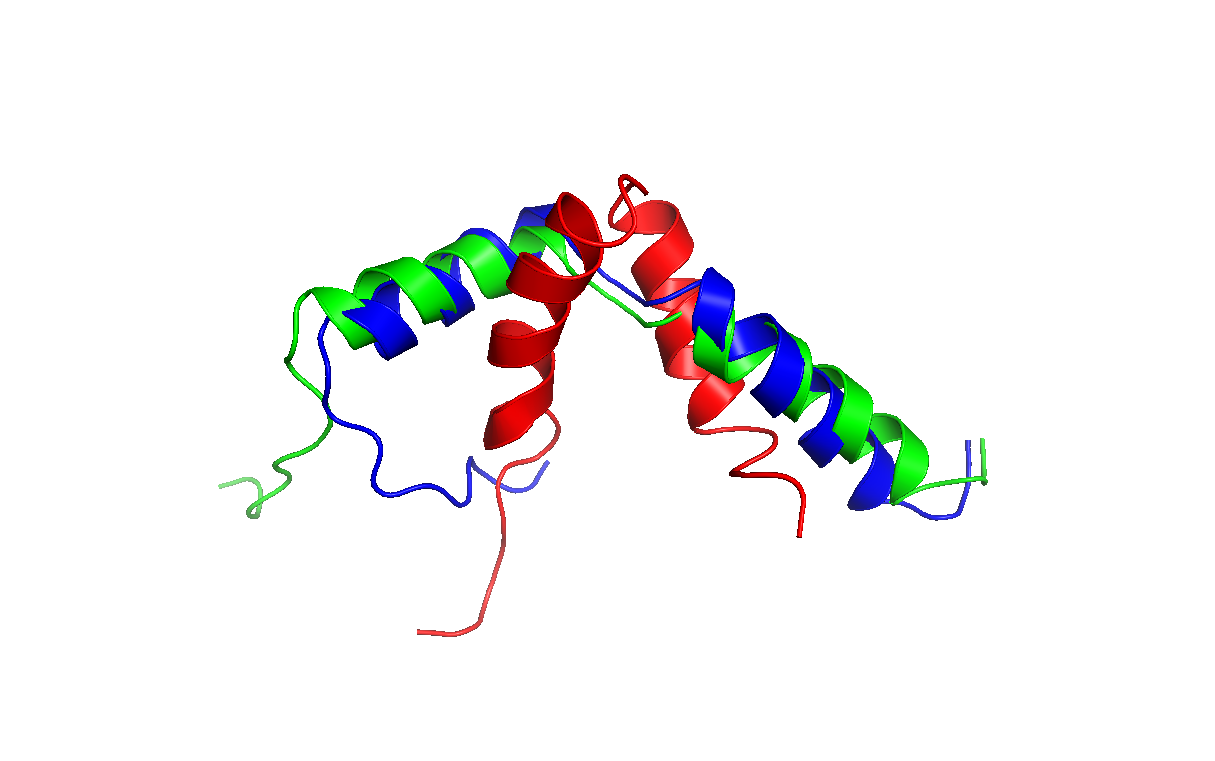
\includegraphics[width=8.5cm]{images/2P81.png} & 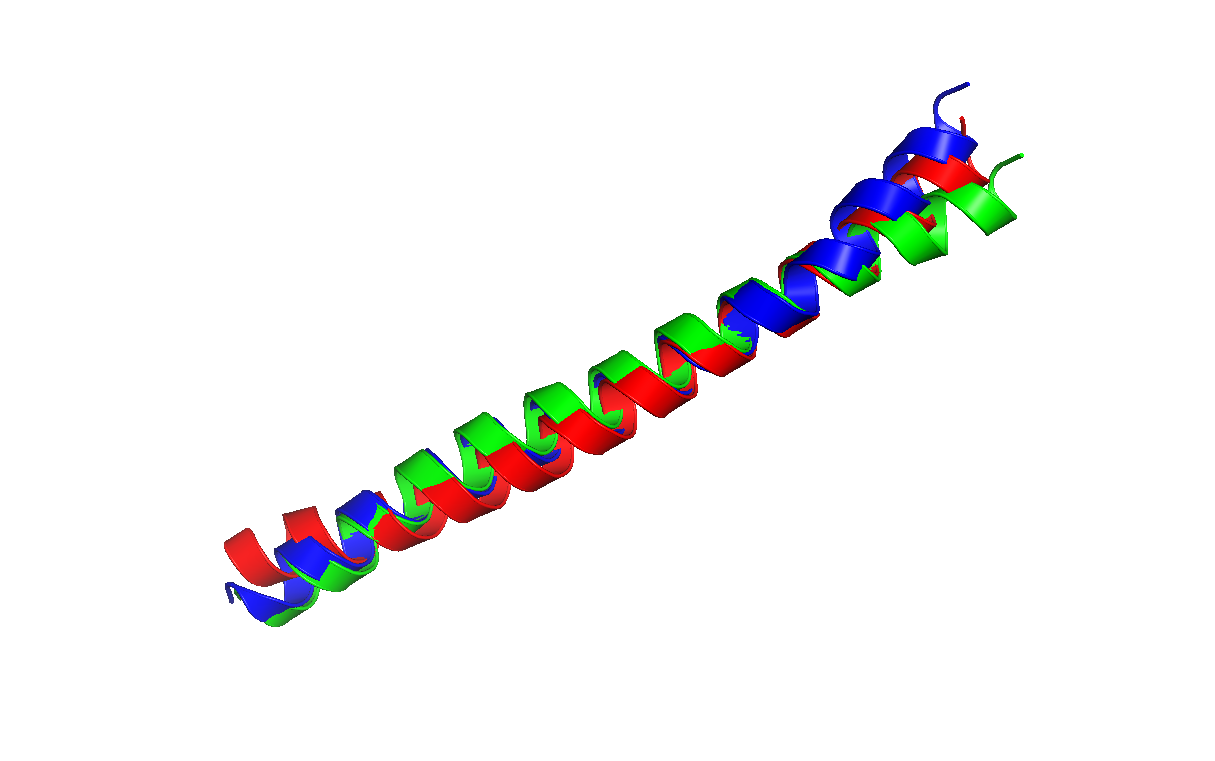
\includegraphics[width=8.5cm]{images/3P7K.png} \\
(e) & (f)\\
\end{tabular}
\caption[Alineación espacial de estructuras extensas]{Resultados de alineación espacial para las proteínas (a) 2F4K, (b) 2JUC, (c) 2MR9, (d) 2P5K, (e) 2P81 y (f) 3P7K. Solución con mejor energía en color verde, mejor RMSD en azul y estructura experimental en rojo. Las estructuras fueron alineadas a partir de la superposición de sus $C_{\alpha}$ utilizando PyMol.}
\label{fig:prot-ext-1}
\end{figure}

\begin{figure}
\centering
\begin{tabular}{c}
\\
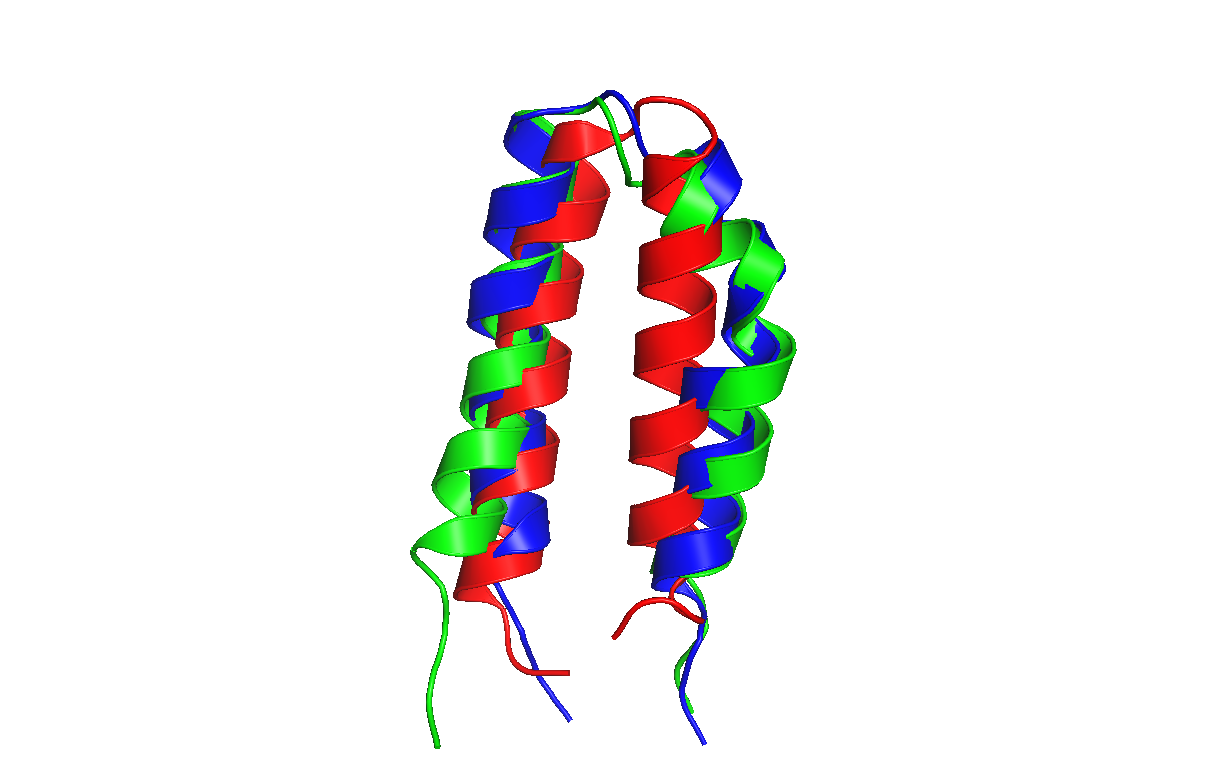
\includegraphics[width=8.5cm]{images/3V1A.png} \\
(g)\\
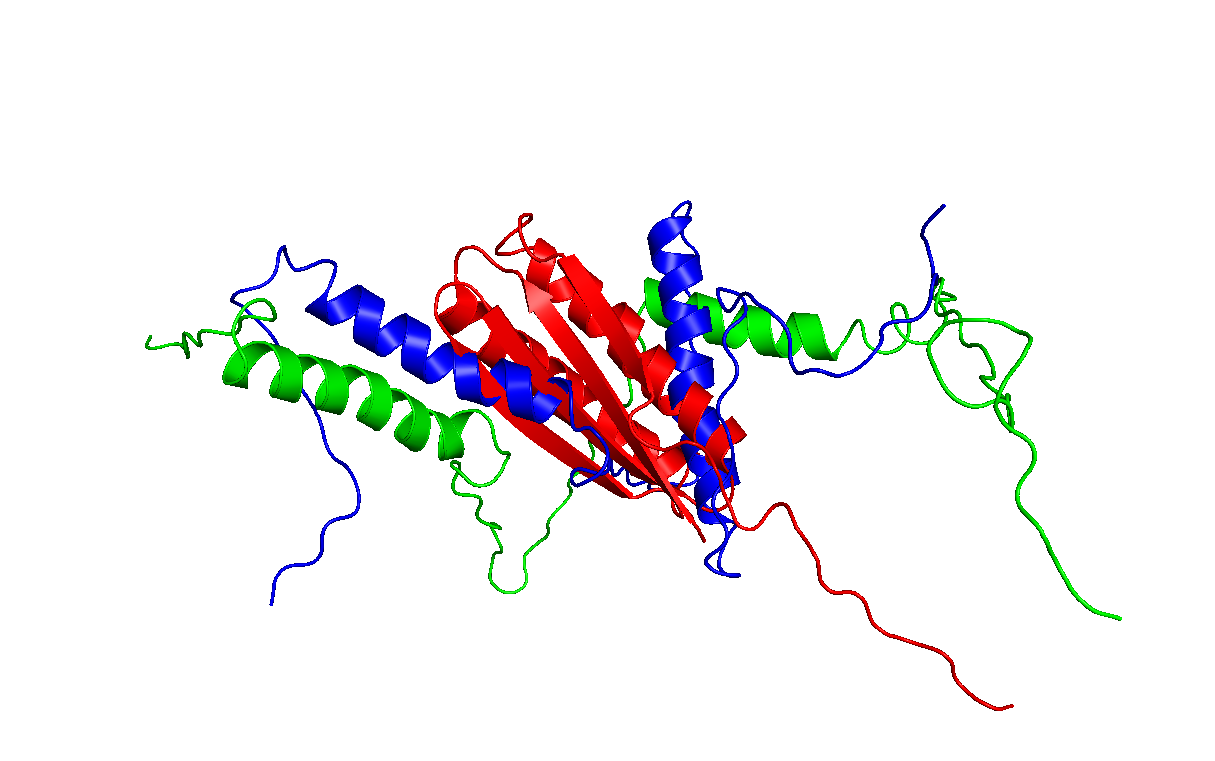
\includegraphics[width=8.5cm]{images/2MQ8.png} \\
(h)\\
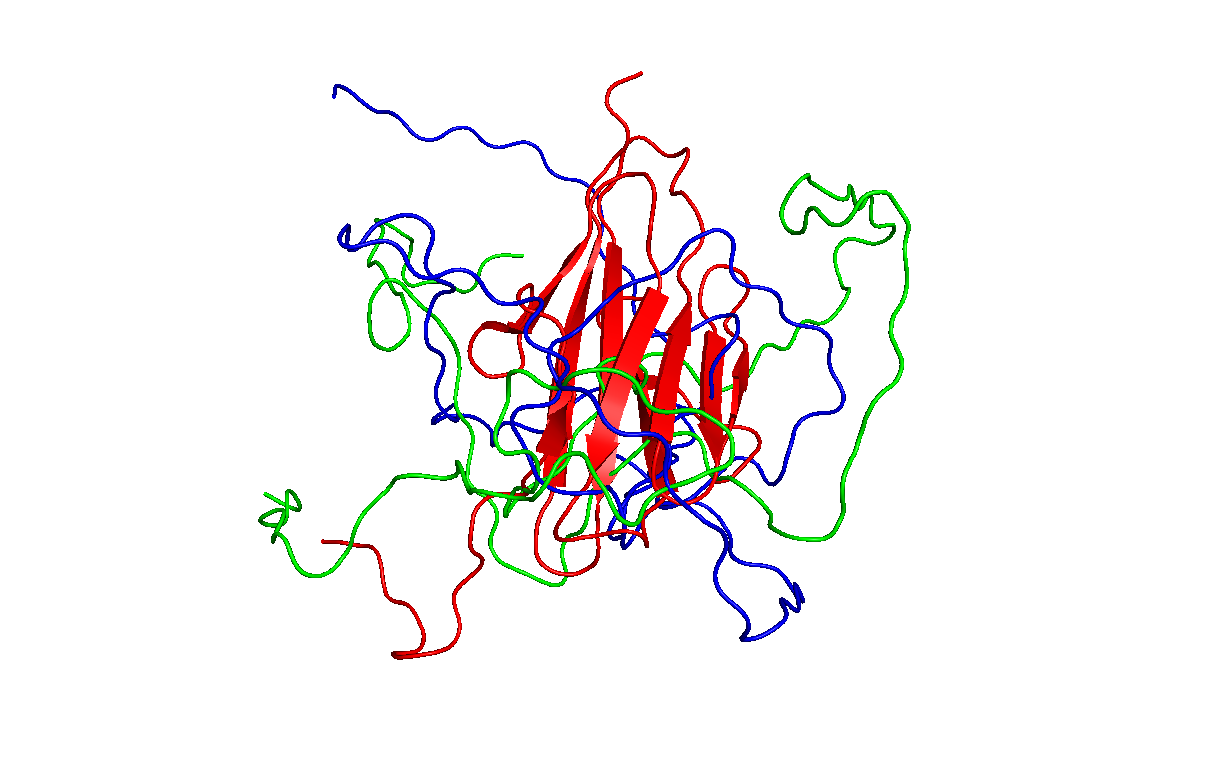
\includegraphics[width=8.5cm]{images/2MW1.png} \\
(i)\\
\end{tabular}
\caption[Alineación espacial de estructuras extensas]{Resultados de alineación espacial para las proteínas (g) 3V1A, (h) 2MQ8 e (i) 2MW1. Solución con mejor energía en color verde, mejor RMSD en azul y estrcutura experimental en rojo. Las estructuras fueron alineadas a partir de la superposición de sus $C_{\alpha}$ utilizando PyMol.}
\label{fig:prot-ext-2}
\end{figure}

Si bien, el MA a nivel de energía continúa encontrado buenas soluciones (energías bajas), sigue evidenciando el problema de predicción de las áreas de curvatura y hojas-$\beta$, no asi con las estructuras tipo hélices que se logran predecir de manera correcta.

Note que las proteínas 2MQ8 y 2MW1 son las más extensas y 72 horas fue tiempo insuficiente para su ejecución, debido a que no lograron llegar a las 50 generaciones. Queda expuesto de forma empírica que el incremento sustancial de aminoácidos en la secuencia implica un costo computacional elevado.
